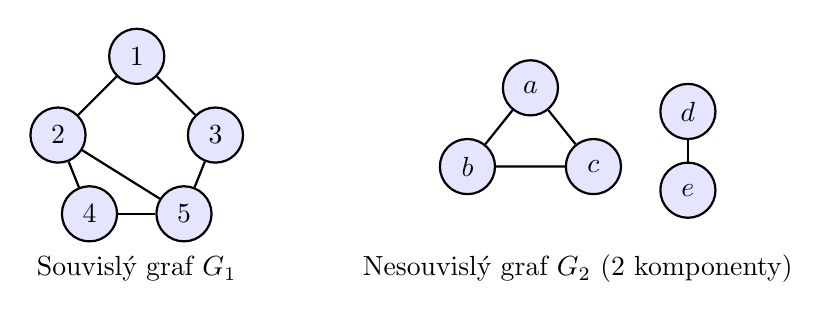
\begin{tikzpicture}[
  vnode/.style={circle, draw, minimum size=7mm, inner sep=0pt, fill=blue!10},
  thick
]
  % Souvislý graf G1 (vlevo)
  \begin{scope}[shift={(-3,0)}]
    \node[vnode] (1) at (0, 1.2) {1};
    \node[vnode] (2) at (-1, 0.2) {2};
    \node[vnode] (3) at (1, 0.2) {3};
    \node[vnode] (4) at (-0.6, -0.8) {4};
    \node[vnode] (5) at (0.6, -0.8) {5};
    \draw (1) -- (2); \draw (1) -- (3); \draw (2) -- (4); \draw (3) -- (5); \draw (4) -- (5); \draw (2) -- (5);
    \node at (0, -1.5) {Souvislý graf $G_1$};
  \end{scope}

  % Nesouvislý graf G2 (vpravo)
  \begin{scope}[shift={(3,0)}]
    % Komponenta A
    \node[vnode] (a) at (-1, 0.8) {$a$};
    \node[vnode] (b) at (-1.8, -0.2) {$b$};
    \node[vnode] (c) at (-0.2, -0.2) {$c$};
    \draw (a) -- (b) -- (c) -- (a);
    
    % Komponenta B
    \node[vnode] (d) at (1, 0.5) {$d$};
    \node[vnode] (e) at (1, -0.5) {$e$};
    \draw (d) -- (e);
    
    \node at (-0.4, -1.5) {Nesouvislý graf $G_2$ (2 komponenty)};
  \end{scope}
\end{tikzpicture}
\par\medskip
\textit{Obrázek 1.1: Ukázka souvislého grafu $G_1$ a nesouvislého grafu $G_2$ s dvěma komponentami indukovanými množinami $\{a,b,c\}$ a $\{d,e\}$.}